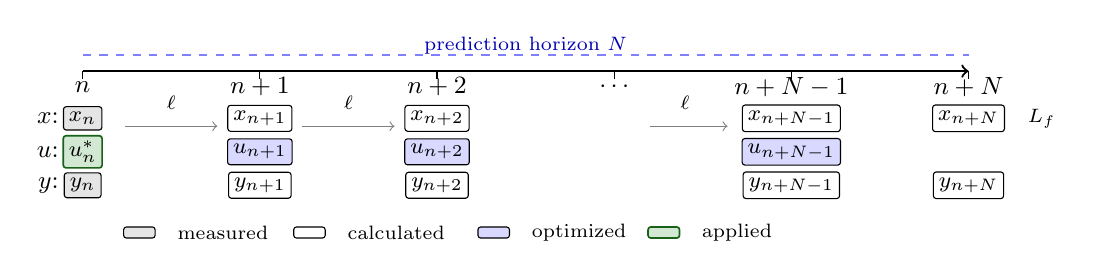
\begin{tikzpicture}[
    time/.style={font=\small},
    var/.style={font=\footnotesize, inner sep=2pt, draw, rounded corners=1pt},
    known/.style={fill=gray!20},
    calc/.style={fill=white},
    opt/.style={fill=blue!15},
    applied/.style={fill=ForestGreen!20, draw=ForestGreen!70!black, line width=0.6pt},
    horizon/.style={dashed, thick, draw=blue!50},
    x=0.9cm, y=0.5cm
]
    % Prediction horizon - above timeline
    \draw[horizon] (0, 2.6) -- (12.5, 2.6);
    \node[font=\scriptsize, blue!70!black] at (6.25, 2.85) {prediction horizon $N$};
    % Timeline
    \draw[->, thick] (0,2.2) -- (12.5,2.2);
    \foreach \x/\lbl in {0/n, 2.5/n+1, 5/n+2, 7.5/\cdots, 10/n+N-1, 12.5/n+N} {
        \draw (\x,2.2) -- (\x,2.0);
        \node[time] at (\x,1.8) {$\lbl$};
    }
    % State row (y=1.0)
    \node[time, anchor=east] at (-0.2, 1.0) {$\boldsymbol{x}$:};
    \node[var, known] at (0, 1.0) {$\boldsymbol{x}_n$};
    \node[var, calc] at (2.5, 1.0) {$\boldsymbol{x}_{n+1}$};
    \node[var, calc] at (5, 1.0) {$\boldsymbol{x}_{n+2}$};
    \node[var, calc] at (10, 1.0) {$\boldsymbol{x}_{n+N-1}$};
    \node[var, calc] at (12.5, 1.0) {$\boldsymbol{x}_{n+N}$};
    % Control row (y=0.15) - more room below x
    \node[time, anchor=east] at (-0.2, 0.15) {$\boldsymbol{u}$:};
    \node[var, applied] at (0, 0.15) {$\boldsymbol{u}_n^*$};
    \node[var, opt] at (2.5, 0.15) {$\boldsymbol{u}_{n+1}$};
    \node[var, opt] at (5, 0.15) {$\boldsymbol{u}_{n+2}$};
    \node[var, opt] at (10, 0.15) {$\boldsymbol{u}_{n+N-1}$};
    % Output row (y=-0.7) - more room below u (u-y gap larger than x-u)
    \node[time, anchor=east] at (-0.2, -0.7) {$\boldsymbol{y}$:};
    \node[var, known] at (0, -0.7) {$\boldsymbol{y}_n$};
    \node[var, calc] at (2.5, -0.7) {$\boldsymbol{y}_{n+1}$};
    \node[var, calc] at (5, -0.7) {$\boldsymbol{y}_{n+2}$};
    \node[var, calc] at (10, -0.7) {$\boldsymbol{y}_{n+N-1}$};
    \node[var, calc] at (12.5, -0.7) {$\boldsymbol{y}_{n+N}$};
    % Cost labels - between timeline and state row
    \node[font=\scriptsize] at (1.25, 1.4) {$\ell$};
    \node[font=\scriptsize] at (3.75, 1.4) {$\ell$};
    \node[font=\scriptsize] at (8.5, 1.4) {$\ell$};
    \node[font=\scriptsize, anchor=west] at (13.2, 1.0) {$L_f$};
    % Dynamics arrows (x_i, u_i) -> x_{i+1}
    \draw[->, gray, thin] (0.6, 0.8) -- (1.9, 0.8);
    \draw[->, gray, thin] (3.1, 0.8) -- (4.4, 0.8);
    \draw[->, gray, thin] (8.0, 0.8) -- (9.1, 0.8);
    % Legend
    \node[var, known, minimum width=0.4cm] at (0.8, -1.9) {};
    \node[font=\scriptsize, anchor=west] at (1.2, -1.9) {measured};
    \node[var, calc, minimum width=0.4cm] at (3.2, -1.9) {};
    \node[font=\scriptsize, anchor=west] at (3.6, -1.9) {calculated};
    \node[var, opt, minimum width=0.4cm] at (5.8, -1.9) {};
    \node[font=\scriptsize, anchor=west] at (6.2, -1.9) {optimized};
    \node[var, applied, minimum width=0.4cm] at (8.2, -1.9) {};
    \node[font=\scriptsize, anchor=west] at (8.6, -1.9) {applied};
\end{tikzpicture}
